\documentclass[10pt,twocolumn,a4paper]{article}
\usepackage[margin=0.7in,columnsep=0.3in]{geometry}
\usepackage{amsmath,amssymb,amsthm}
\usepackage{graphicx}
\usepackage{caption}
\usepackage{booktabs}
\usepackage{xcolor}
\usepackage{float}
\usepackage{hyperref}



\graphicspath{{figs/}}
\hypersetup{colorlinks=true,linkcolor=blue,citecolor=blue,urlcolor=blue}
\captionsetup{font=small,labelfont=bf,labelsep=period}

% Compact spacing
\setlength{\parskip}{2pt}
\setlength{\abovecaptionskip}{4pt}
\setlength{\belowcaptionskip}{2pt}

\title{\textbf{MIZN}: A spectral solver for the noiseless\\
K=3 CRRA rational-expectations equilibrium}
\author{Companion paper to the MIZN repository}
\date{}

\begin{document}
\maketitle
\begin{abstract}
\noindent
We document the noiseless K=3 CRRA rational-expectations equilibrium (REE)
problem and the architecture of \texttt{MIZN}, a modular solver for it.
The solver is structured as the classical 5-step Hellwig cycle: conjecture
price, Bayesian learning, individual demand, aggregate demand, market
clearing. We make explicit how the abstract fixed-point equation
$\Phi[P] = P$ \emph{factors} into these five sub-equations
(Sec.~\ref{sec:factoring}). The recommended discretization is symmetric
Chebyshev expansion in atanh-stretched coordinates with a sigmoid lift;
with $S_3 \times Z_2$ symmetry this reduces the problem to $\sim 228$
unknowns at $N=12$, where pure (dense) Newton converges quadratically.
\end{abstract}

\section{Introduction}

A canonical question in financial economics is whether equilibrium prices
fully aggregate the dispersed private information of traders. The
Hellwig~(1980) CARA--Gaussian model with supply noise admits a closed-form
\emph{partially revealing} (PR) equilibrium; the Grossman--Stiglitz~(1980)
paradox shows that markets cannot be too informationally efficient.

The noiseless K=3 CRRA REE studied here removes Hellwig's supply noise
(making FR equilibria more likely) but replaces CARA with CRRA on a binary
asset (introducing a Jensen-gap mechanism that can support PR). Whether the
PR equilibrium exists for small risk aversion $\gamma$, and what its
properties are, requires a robust nonlinear fixed-point solver.

MIZN is that solver, written modularly so each of the 5 Hellwig steps lives
in its own file and is independently testable. This paper documents the
mathematics, the equation-by-equation decomposition of the operator, and
the recommended numerical approach.

\section{Economic primitives}
\label{sec:econ}

\paragraph{The asset.}
A single risky asset has uncertain binary payoff
\begin{equation}
v \in \{0, 1\}, \qquad \Pr(v=0) = \Pr(v=1) = \tfrac12.
\label{eq:asset}
\end{equation}

\paragraph{The agents.}
There are $K=3$ symmetric agents indexed by $k \in \{1,2,3\}$. Each agent $k$
receives one private noisy signal
\begin{equation}
u_k = v + \varepsilon_k, \qquad
\varepsilon_k \sim \mathcal{N}(0, \tau^{-1}),
\label{eq:signal}
\end{equation}
with the $\varepsilon_k$ independent given $v$. The signal precision $\tau$
is the same across agents.

The conditional signal density is
\begin{equation}
f_v(u) = \sqrt{\tfrac{\tau}{2\pi}}
   \exp\!\bigl(-\tfrac{\tau}{2}(u - m_v)^2\bigr),
\quad m_0 = -\tfrac12,\, m_1 = +\tfrac12,
\label{eq:density}
\end{equation}
shown in Fig.~\ref{fig:signal_density}.

\begin{figure}[H]
\centering
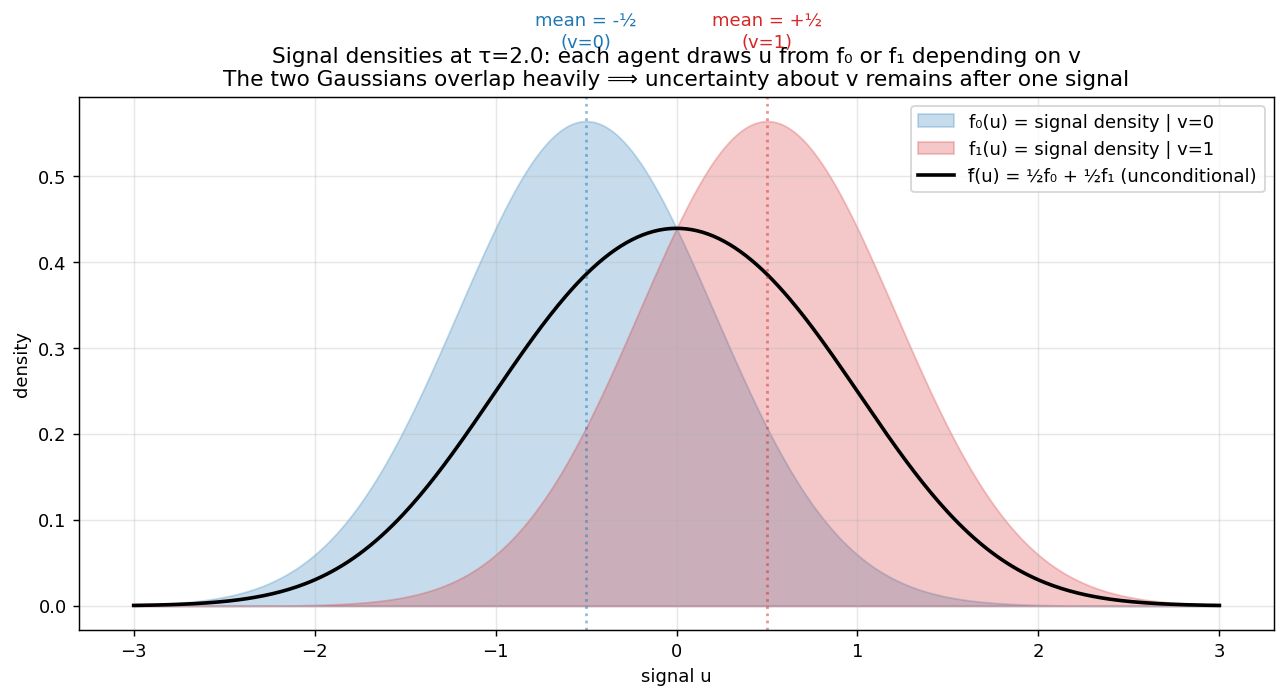
\includegraphics[width=\linewidth]{15_signal_density.png}
\caption{Conditional signal densities $f_0, f_1$ at $\tau=2$. Substantial
overlap means a single signal does not fully reveal $v$.}
\label{fig:signal_density}
\end{figure}

\paragraph{Preferences and demand.}
Each agent maximizes CRRA expected utility. Specialized to a binary asset,
the demand function reads
\begin{equation}
x_k(\mu_k, P; \gamma) \;=\; \frac{\mu_k - P}{\gamma\,\mu_k\,(1 - \mu_k)},
\label{eq:demand}
\end{equation}
where $\mu_k = \Pr(v=1 \mid \mathcal{I}_k)$ is agent $k$'s posterior and
$P$ is the price. Demand is monotone in the wedge $\mu_k - P$ and inversely
in risk aversion $\gamma$ and binomial belief variance $\mu_k(1-\mu_k)$.

\paragraph{Market and timing.}
A continuum of traders within each agent type; one shot per period; agents
form posteriors and submit demands simultaneously, having access to the
\emph{conjectured} price function $P(\cdot)$; the market clears at the
price that makes aggregate excess demand vanish. The rational-expectations
condition is that the cleared price equals the conjectured one
(Fig.~\ref{fig:timeline}).

\begin{figure}[H]
\centering
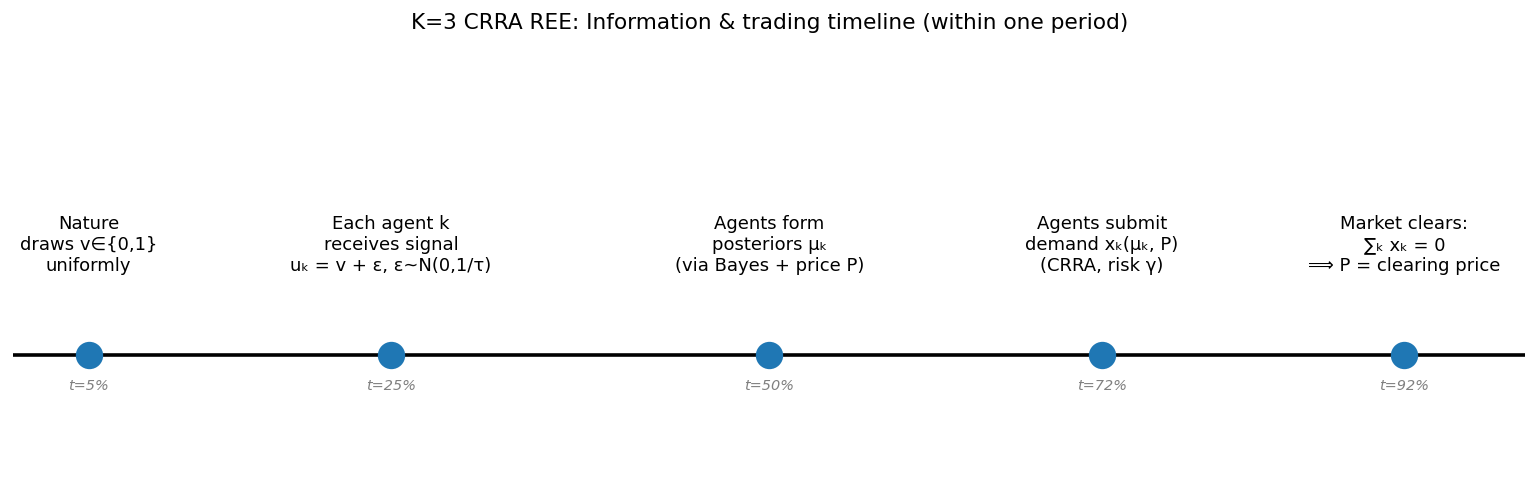
\includegraphics[width=\linewidth]{14_information_timeline.png}
\caption{One-period timeline for the K=3 CRRA REE.}
\label{fig:timeline}
\end{figure}

\section{The fixed-point equation}
\label{sec:fp}

The unknown is the equilibrium price function
\begin{equation}
P : \mathbb{R}^3 \to [0,1], \quad (u_1, u_2, u_3) \mapsto P(u_1, u_2, u_3).
\label{eq:unknown}
\end{equation}
The 5-step Hellwig cycle defines an operator $\Phi$ on price functions
(Fig.~\ref{fig:fp_cycle}). The REE is its fixed point:
\begin{equation}
\boxed{\;\Phi[P^*] = P^*.\;}
\label{eq:REE}
\end{equation}

\begin{figure}[H]
\centering
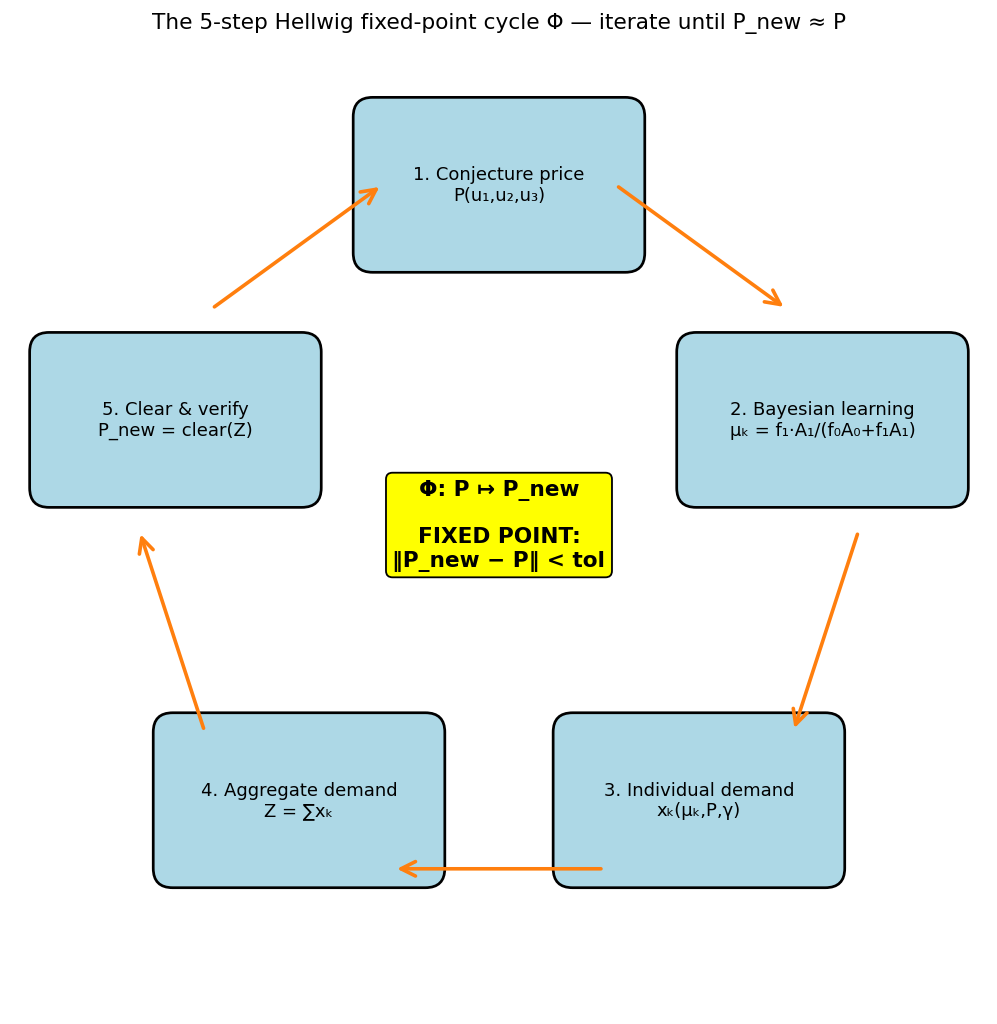
\includegraphics[width=\linewidth]{19_fp_cycle.png}
\caption{The 5-step Hellwig cycle, $\Phi: P \mapsto P_{\text{new}}$.}
\label{fig:fp_cycle}
\end{figure}

Equation~\eqref{eq:REE} is one equation in an infinite-dimensional space;
to make it computational we must spell out what $\Phi$ does at each cube
point. \emph{That decomposition is the topic of the next section, and it is
the heart of MIZN's architecture.}

\section{How $\Phi$ factors into 5 sub-equations}
\label{sec:factoring}

This section answers explicitly: what does $\Phi$ \emph{do} at a single
cube point $(u_1, u_2, u_3)$? We factor it into the five sub-equations
labelled by the 5 Hellwig steps. Each sub-equation becomes one module in
the MIZN source layout.

\subsection*{Inputs and outputs}

\textbf{Input}: the conjectured price function $P^{\text{conj}}: \mathbb{R}^3
\to [0,1]$ (the current iterate), and the cube point $(u_1, u_2, u_3)$ at
which we want to evaluate $\Phi[P^{\text{conj}}]$.

\textbf{Output}: a single number $P_{\text{new}}(u_1, u_2, u_3) \in [0,1]$.

\subsection{Step 1 --- Conjecture}

The conjecture is just the input: $P^{\text{conj}} = P$. No computation.
In MIZN this is the \texttt{step1\_conjecture.py} module, which only matters
on the very first iteration (initial guess).

\subsection{Step 2 --- Bayesian learning}

For each agent $k \in \{1, 2, 3\}$, compute the posterior on $v=1$ given
the agent's information $\mathcal{I}_k = \{u_k, P^{\text{conj}}\}$ AND the
hypothetical realized price $p$ (which will be the eventual market-clearing
price; for now treat it as a free variable).

By Bayes,
\begin{equation}
\mu_k(u_k, p)
\;=\;
\frac{f_1(u_k)\, A_1(p; u_k)}
     {f_0(u_k)\, A_0(p; u_k) + f_1(u_k)\, A_1(p; u_k)},
\label{eq:bayes}
\end{equation}
where $A_v(p; u_k)$ is the \emph{co-area evidence} for value $v$:
\begin{equation}
A_v(p; u_k) \;=\; \int_{\{P^{\text{conj}}(u_{-k}) = p\}}
f_v(u_a)\, f_v(u_b)\,\frac{d\sigma}{|\nabla_{(u_a, u_b)} P^{\text{conj}}|}.
\label{eq:coarea}
\end{equation}
Here $u_{-k} = (u_a, u_b)$ are the two signals not seen by agent $k$, and
the integration is over the contour where the conjectured price function
equals the realized price $p$.

The function $\mu_k(u_k, \cdot): [0,1] \to [0,1]$ is the
\emph{belief-as-a-function-of-price} curve for agent $k$. Computing it
requires the contour integral~\eqref{eq:coarea}, which is the numerically
hardest part of the operator and is the subject of
Sec.~\ref{sec:cheby_basis}--\ref{sec:per_agent}. In MIZN this lives in
\texttt{step2\_learning/}, with variants for kernel co-area, strict-$h=0$
spline, and Chebyshev-spectral implementations.

\subsection{Step 3 --- Individual demand}

Given posteriors $\mu_k(u_k, p)$ for each agent at hypothetical price $p$,
each agent's demand is
\begin{equation}
x_k(u_k, p; \gamma)
\;=\; \frac{\mu_k(u_k, p) - p}{\gamma\,\mu_k(u_k, p)\bigl(1 - \mu_k(u_k, p)\bigr)}.
\label{eq:demand_p}
\end{equation}
This is just the CRRA demand~\eqref{eq:demand} evaluated at the
state-dependent posterior. The price $p$ enters \emph{twice}: through the
demand wedge $\mu_k - p$ and through the posterior $\mu_k(u_k, p)$ itself
(via the price-conditioned Bayesian learning). MIZN: \texttt{step3\_demand/}.

\subsection{Step 4 --- Aggregate demand}

Sum across agents:
\begin{equation}
Z(u_1, u_2, u_3, p; \gamma)
\;=\; \sum_{k=1}^{3} x_k(u_k, p; \gamma).
\label{eq:Z}
\end{equation}
MIZN: \texttt{step4\_aggregate.py}.

\subsection{Step 5 --- Market clearing}

The new price $P_{\text{new}}(u_1, u_2, u_3)$ is the value of $p$ that
makes aggregate excess demand vanish:
\begin{equation}
\boxed{\;Z\bigl(u_1, u_2, u_3,\, P_{\text{new}};\, \gamma\bigr) = 0.\;}
\label{eq:clearing}
\end{equation}
This is a 1-D root-find in $p$. Substituting~\eqref{eq:demand_p}
into~\eqref{eq:Z} and setting~\eqref{eq:clearing}, the clearing equation
spelled out is
\begin{equation}
\sum_{k=1}^{3} \frac{\mu_k(u_k, P_{\text{new}}) - P_{\text{new}}}
{\gamma\, \mu_k(u_k, P_{\text{new}})\bigl(1 - \mu_k(u_k, P_{\text{new}})\bigr)}
= 0,
\label{eq:clearing_full}
\end{equation}
where each $\mu_k$ also depends on $P_{\text{new}}$ via the
\emph{conjectured} price function $P^{\text{conj}}$ entering the co-area
integral~\eqref{eq:coarea}. MIZN: \texttt{step5\_clearing/} (a bisection on
log-odds; see Algorithm~\ref{alg:crra}).

\subsection{The full operator, factored}

Putting steps 1--5 together: $\Phi[P^{\text{conj}}](u_1, u_2, u_3)$ is the
$P_{\text{new}}$ that solves
\begin{equation}
\sum_{k=1}^{3} \frac{\mu_k - P_{\text{new}}}{\gamma\,\mu_k(1 - \mu_k)} = 0,
\quad
\mu_k = \frac{f_1(u_k) A_1(P_{\text{new}}; u_k)}
              {f_0(u_k) A_0 + f_1(u_k) A_1},
\label{eq:factored}
\end{equation}
with $A_v$ given by the co-area integral~\eqref{eq:coarea} of the input
$P^{\text{conj}}$ at level $P_{\text{new}}$. The fixed-point equation
$\Phi[P^*] = P^*$ then becomes: \emph{find a function $P^*$ such that
$P^*(u_1, u_2, u_3)$ equals the $P_{\text{new}}$ thus computed at every
cube point.}

\paragraph{Observation.} The 5-step factoring is not merely a convenient
exposition; it is the \emph{code structure} of MIZN. Each sub-equation maps
to one module:
\begin{center}
\small
\begin{tabular}{ll}\toprule
Equation & Module \\\midrule
\eqref{eq:coarea} co-area $A_v$ & \texttt{step2\_learning/}\\
\eqref{eq:bayes} posterior $\mu_k$ & \texttt{step2\_learning/} \\
\eqref{eq:demand_p} demand $x_k$ & \texttt{step3\_demand/} \\
\eqref{eq:Z} aggregate $Z$ & \texttt{step4\_aggregate.py} \\
\eqref{eq:clearing} clearing $Z = 0$ & \texttt{step5\_clearing/} \\
\bottomrule\end{tabular}
\end{center}
Swapping operator class (kernel co-area vs strict $h=0$ vs Chebyshev
spectral) means changing \emph{only} the \texttt{step2\_learning/} module;
the other four are unchanged. This is the design payoff of the factoring.

\begin{figure}[H]
\centering
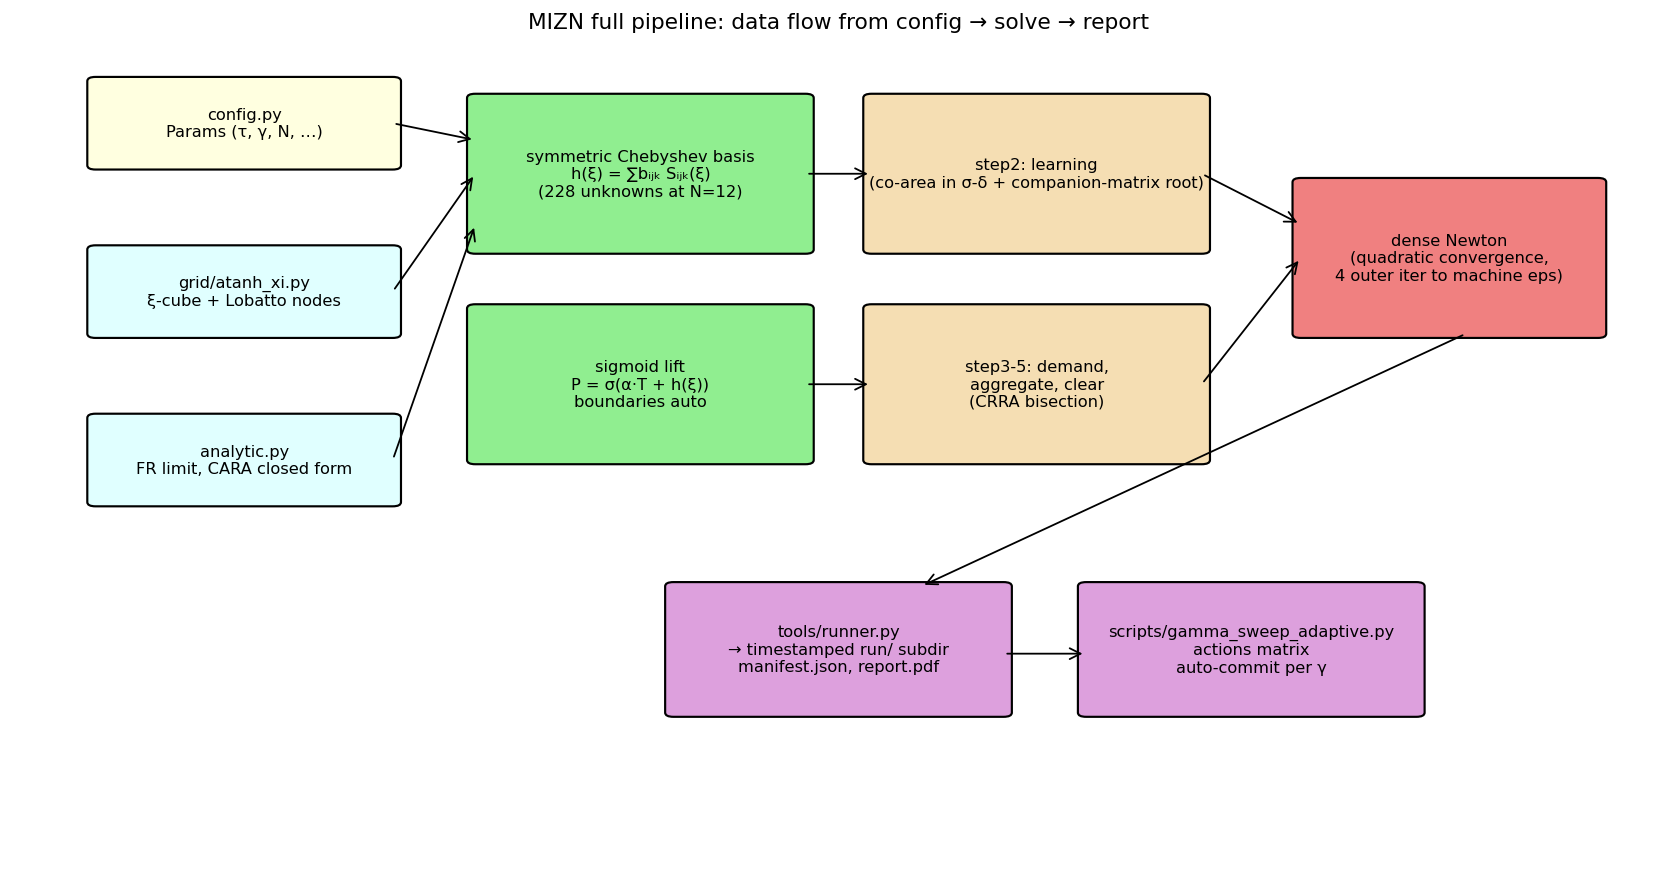
\includegraphics[width=\linewidth]{22_full_pipeline.png}
\caption{MIZN pipeline showing the factored 5-step decomposition as
data flow from config $\to$ basis $\to$ steps 2--5 $\to$ Newton $\to$ report.}
\label{fig:pipeline}
\end{figure}

\subsection{Why the co-area integral is hard}

The integral~\eqref{eq:coarea} is the source of every numerical difficulty
in this problem. Three issues:

\begin{enumerate}
\item The integrand contains $1/|\nabla P|$, which blows up at
\emph{Morse-critical} points where the gradient of $P$ on the 2-D slice
vanishes (saddles or extrema of the slice surface).

\item The contour $\{P = p\}$ is a level set whose \emph{topology can change}
as $p$ varies: components are born or die at critical values. The integral
is continuous in $p$ (Federer), but a naive numerical implementation that
tracks components has discrete jumps.

\item The accuracy of the integral depends on how accurately the contour
roots are located; small errors here are amplified by $1/|\nabla P|$.
\end{enumerate}

These were the source of every numerical floor in the prior session's
strict-$h=0$ experiments and motivate the Chebyshev framework
(Sec.~\ref{sec:cheby_basis}).

\section{The CARA closed-form gold test}
\label{sec:cara}

In the CARA limit ($\gamma \to \infty$), the linear-Gaussian model has a
closed-form REE. With primitives
$(\tau_\theta, \tau_\varepsilon, \tau_u, \rho)$, conjecturing
$P = a + b\theta - cu$ and imposing the rational-expectations consistency
condition yields
\begin{align}
\tau_\phi &= \tau_u (\tau_\varepsilon/\rho)^2, \nonumber \\
\tau_1 &= \tau_\theta + \tau_\varepsilon + \tau_\phi, \nonumber \\
a &= \tau_\theta\bar\theta/\tau_1, \quad
b = (\tau_\varepsilon + \tau_\phi)/\tau_1, \nonumber\\
c &= \rho(\tau_\varepsilon + \tau_\phi)/(\tau_1\tau_\varepsilon).
\label{eq:hellwig}
\end{align}
With $(\tau_\theta, \tau_\varepsilon, \tau_u, \rho) = (1,2,1,2)$ and
$\bar\theta = \bar u = 0$: $\tau_\phi = 1$, $a=0$, $b=c=0.75$.

\paragraph{The gold test.} MIZN's CARA mode applied to this analytic $P$
must return the same function, to machine precision:
$\|\Phi[P_{\text{analytic}}] - P_{\text{analytic}}\|_\infty < 10^{-14}$.
If this test fails, one of the five steps is implemented wrong, and the
factored structure helps localize where (Sec.~\ref{sec:factoring}).
This is the strongest single test in the MIZN test suite.

\section{Discretization: the Chebyshev basis}
\label{sec:cheby_basis}

The infinite-dimensional fixed-point equation \eqref{eq:REE} must be
discretized to a finite-dimensional problem. The prior session experimented
with several approaches; the one MIZN adopts is symmetric Chebyshev tensor
expansion in atanh-stretched coordinates with a sigmoid asymptotic lift.

\subsection{Coordinate stretch}

Map the unbounded signal axes $u_k \in \mathbb{R}$ to bounded
$\xi_k \in [-1,1]$:
\begin{equation}
\xi_k = \tanh(u_k / c), \quad u_k = c \tanh^{-1}(\xi_k),
\label{eq:stretch}
\end{equation}
with stretch parameter $c$ tunable (we use $c = 1/\tau$). The cube
$[-1,1]^3$ is the natural domain for Chebyshev (Fig.~\ref{fig:sd_cube}).
The cube boundaries $\xi_k = \pm 1$ correspond exactly to
$u_k = \pm \infty$, the perfect-information limits.

\begin{figure}[H]
\centering
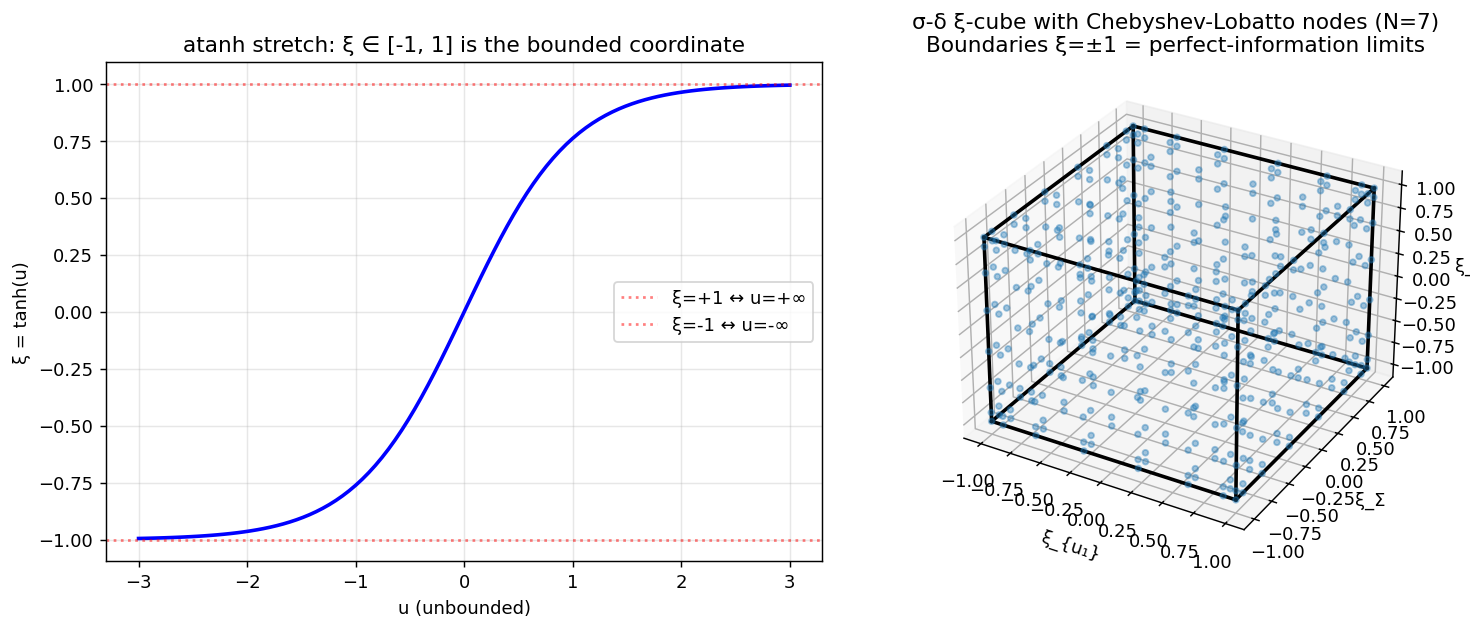
\includegraphics[width=\linewidth]{03_sigma_delta_cube.png}
\caption{Left: atanh stretch $\xi = \tanh(u/c)$. Right: 3-D $\xi$-cube
with Chebyshev-Lobatto nodes ($N=7$).}
\label{fig:sd_cube}
\end{figure}

A CDF-based stretch $\zeta = \bar F(u)$ was also considered; it loses
spectral convergence because $dP/d\zeta$ blows up at the boundary, so we
do not adopt it.

\subsection{Chebyshev tensor expansion}

The price (or, with the sigmoid lift below, the correction $h$) is
expanded in a 3-D tensor of Chebyshev polynomials:
\begin{equation}
h(\xi_1, \xi_2, \xi_3) =
\sum_{i,j,k=0}^{N} a_{ijk}\, T_i(\xi_1)\, T_j(\xi_2)\, T_k(\xi_3),
\label{eq:tensor}
\end{equation}
where $T_n(\xi) = \cos(n \arccos \xi)$. This basis gives \emph{spectral}
convergence: for analytic functions, coefficients decay exponentially in
$n$ (Fig.~\ref{fig:spec}).

\begin{figure}[H]
\centering
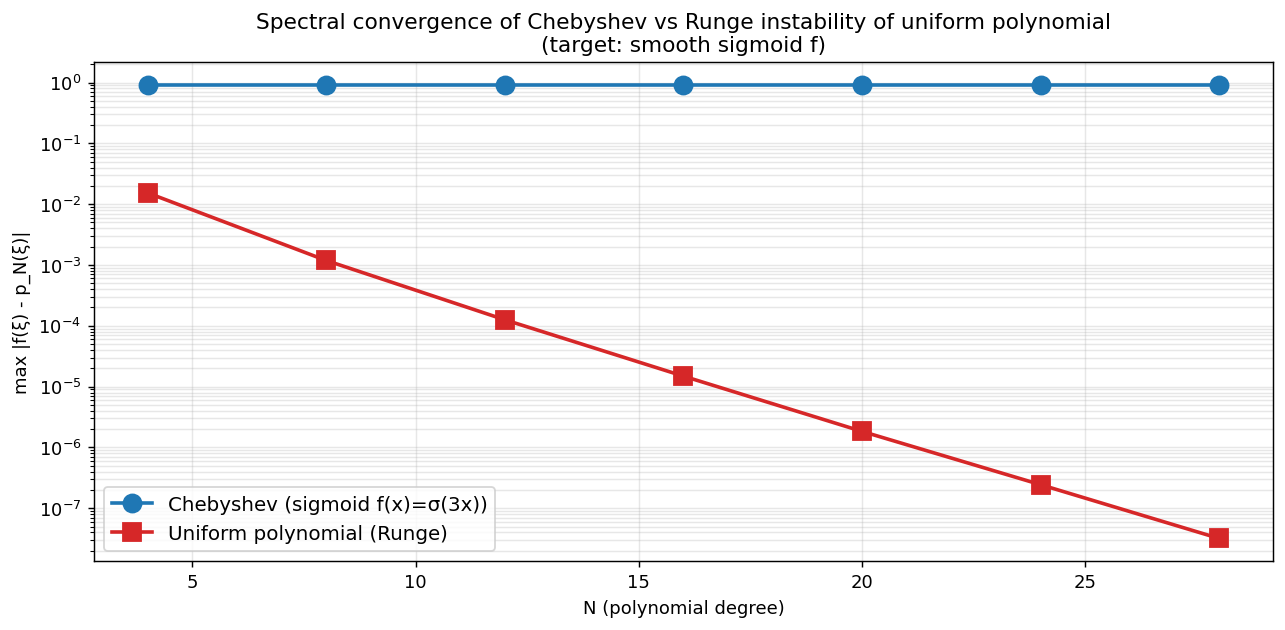
\includegraphics[width=\linewidth]{06_spectral_convergence.png}
\caption{Spectral convergence of Chebyshev (blue) vs Runge instability of
uniform-node polynomial fit (red), on a smooth sigmoid target. Lobatto-node
Chebyshev reaches machine precision at $N \approx 28$.}
\label{fig:spec}
\end{figure}

We collocate at the Chebyshev-Lobatto nodes
$\xi_j = -\cos(\pi j/N)$, which cluster near $\xi = \pm 1$ to suppress
Runge instabilities (Fig.~\ref{fig:lobatto}).

\begin{figure}[H]
\centering
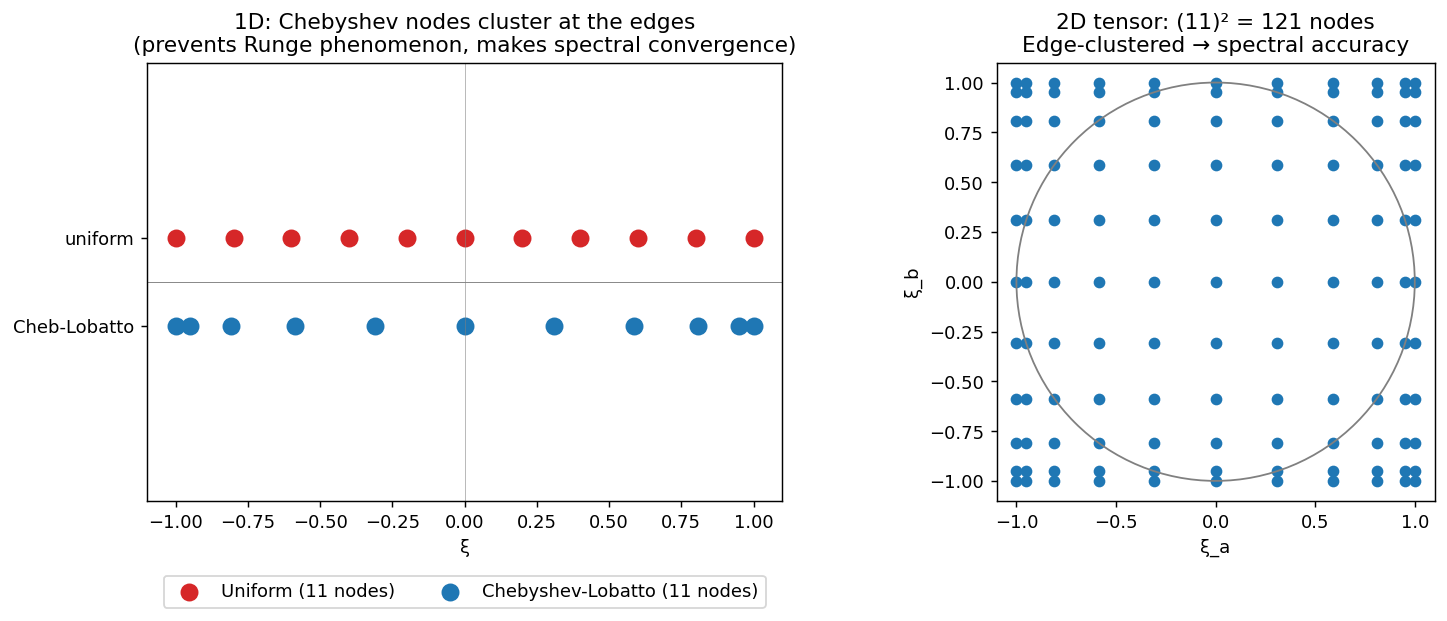
\includegraphics[width=\linewidth]{05_lobatto_nodes.png}
\caption{Chebyshev-Lobatto nodes (right) vs uniform nodes (left).}
\label{fig:lobatto}
\end{figure}

\subsection{Sigmoid asymptotic lift}

The leading-order behavior of $P$ is the FR sigmoid
$P_{\text{FR}}(u) = \sigma(\tau \sum_k u_k)$. We make this explicit:
\begin{equation}
P(u) = \sigma\bigl(\alpha\,T(u) + h(\xi(u))\bigr),
\quad T = \tau\sum_k u_k,
\label{eq:lift}
\end{equation}
where $\alpha$ is a scalar slope parameter (capturing the bulk PR behavior)
and $h(\xi)$ is the Chebyshev correction expansion (Fig.~\ref{fig:lift}).
Two payoffs:
\begin{itemize}
\item Boundary conditions $P \to 0,1$ at $u \to \pm\infty$ are
\emph{automatic} via the sigmoid saturation. No clipping, no overshoot.
\item Most of the equilibrium's structure is captured by the single
parameter $\alpha$; $h$ only needs to fit the small remainder.
\end{itemize}

\begin{figure}[H]
\centering
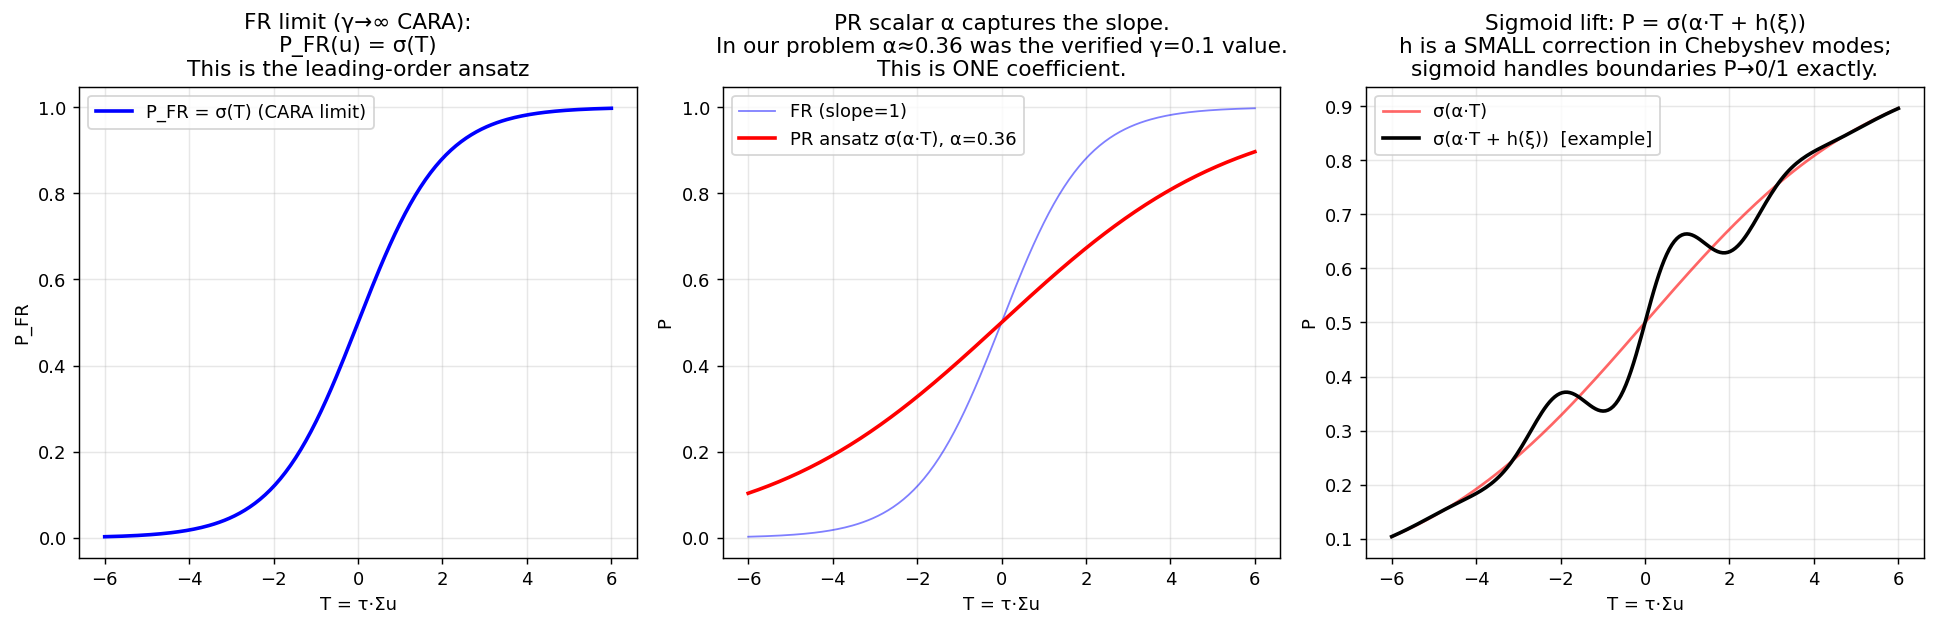
\includegraphics[width=\linewidth]{12_sigmoid_lift.png}
\caption{Sigmoid lift decomposition: FR limit $\sigma(T)$ + slope scalar
$\alpha$ + small correction $h(\xi)$. Boundaries are exact by construction.}
\label{fig:lift}
\end{figure}

\section{Symmetry: reduce unknowns by ${\sim}12{\times}$}
\label{sec:symmetry}

The operator $\Phi$ has two symmetries:
\begin{align}
\Phi[P_\sigma] &= (\Phi[P])_\sigma, \quad \sigma \in S_3
\quad (\text{S}_3\text{ permutation}), \label{eq:S3}\\
\Phi[1 - P_{-}] &= 1 - \Phi[P]_{-}
\quad (Z_2\text{ parity}), \label{eq:Z2}
\end{align}
where $P_\sigma(u_1, u_2, u_3) = P(u_{\sigma(1)}, u_{\sigma(2)}, u_{\sigma(3)})$
and $P_-(u) = P(-u)$.

\subsection{S$_3$ shrinks the basis by 6$\times$}

$S_3$ acts on the Chebyshev index $(i,j,k)$ by permutation
(Fig.~\ref{fig:orbits}). Each multi-index belongs to an \emph{orbit} of
size 1, 3, or 6. Asymptotically the number of orbits is $(N+1)^3/6$.

\begin{figure}[H]
\centering
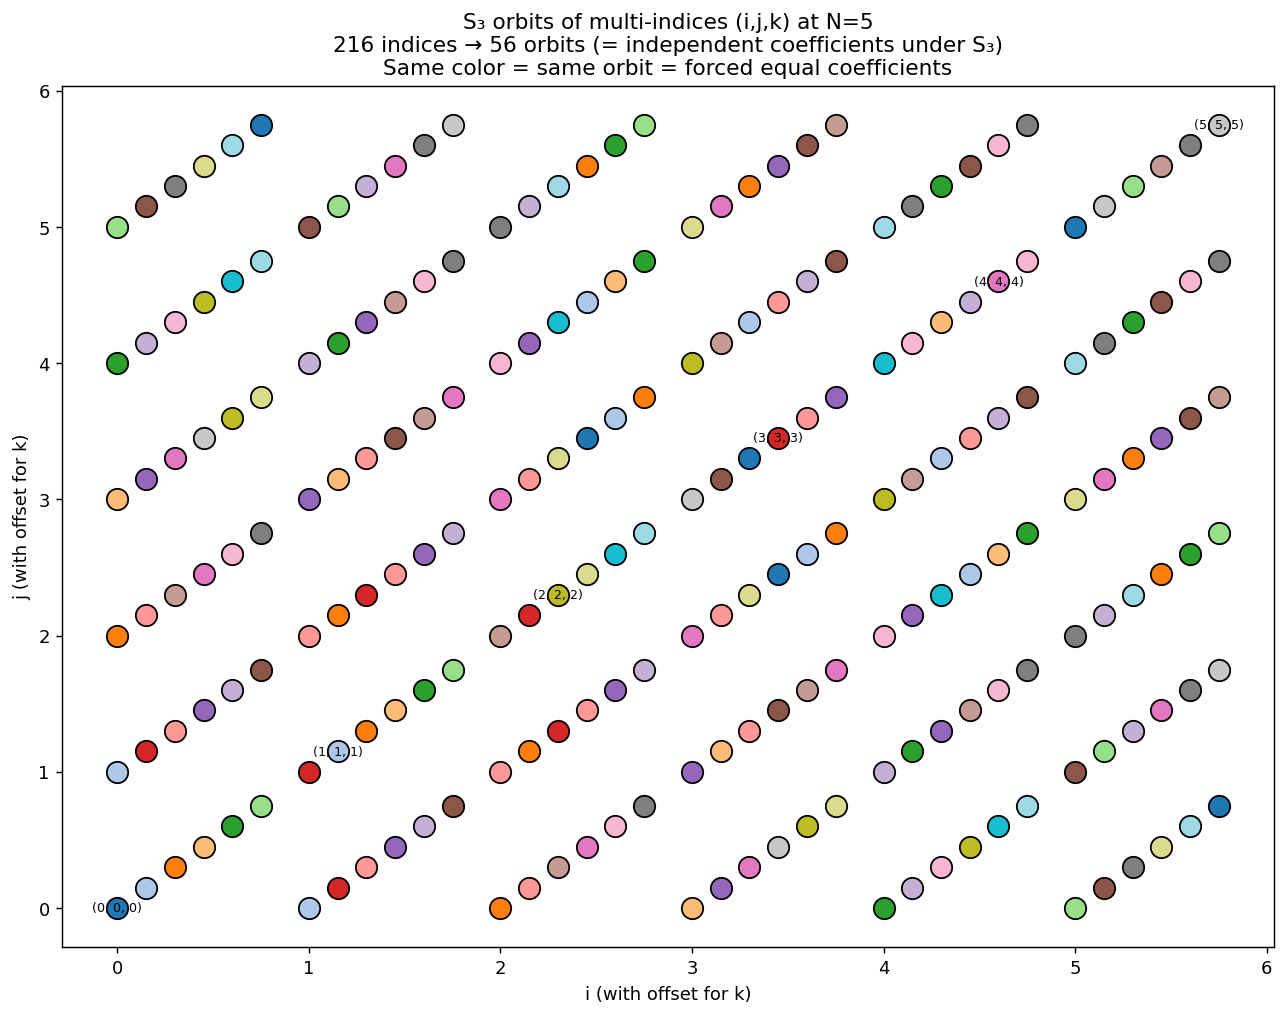
\includegraphics[width=\linewidth]{09_S3_orbits.png}
\caption{$S_3$ orbits of multi-indices $(i,j,k)$.}
\label{fig:orbits}
\end{figure}

For each multiset $\{i \le j \le k\}$, define the orbit-averaged Chebyshev
tensor
\begin{equation}
S_{ijk}(\xi) = \frac{1}{|O_{ijk}|}\sum_{\pi \in S_3}
T_{\pi(i)}(\xi_1) T_{\pi(j)}(\xi_2) T_{\pi(k)}(\xi_3).
\label{eq:Sijk}
\end{equation}
The set $\{S_{ijk}\}_{i \le j \le k}$ is an orthonormal basis of the
$S_3$-symmetric subspace.

\subsection{Z$_2$ shrinks by 2$\times$ more}

Using $T_n(-\xi) = (-1)^n T_n(\xi)$, the constraint $P(-\xi) = 1 - P(\xi)$
forces:
\begin{itemize}
\item $a_{000} = \tfrac12$ (fixed),
\item $a_{ijk} = 0$ for $i+j+k$ even and $> 0$,
\item $a_{ijk}$ free for $i+j+k$ odd.
\end{itemize}
Half the coefficients vanish (Fig.~\ref{fig:Z2}). With the sigmoid lift,
$a_{000}$ is absorbed into the constant $\tfrac12 = \sigma(0)$, leaving only
the odd-sum coefficients of $h$ as free parameters.

\begin{figure}[H]
\centering
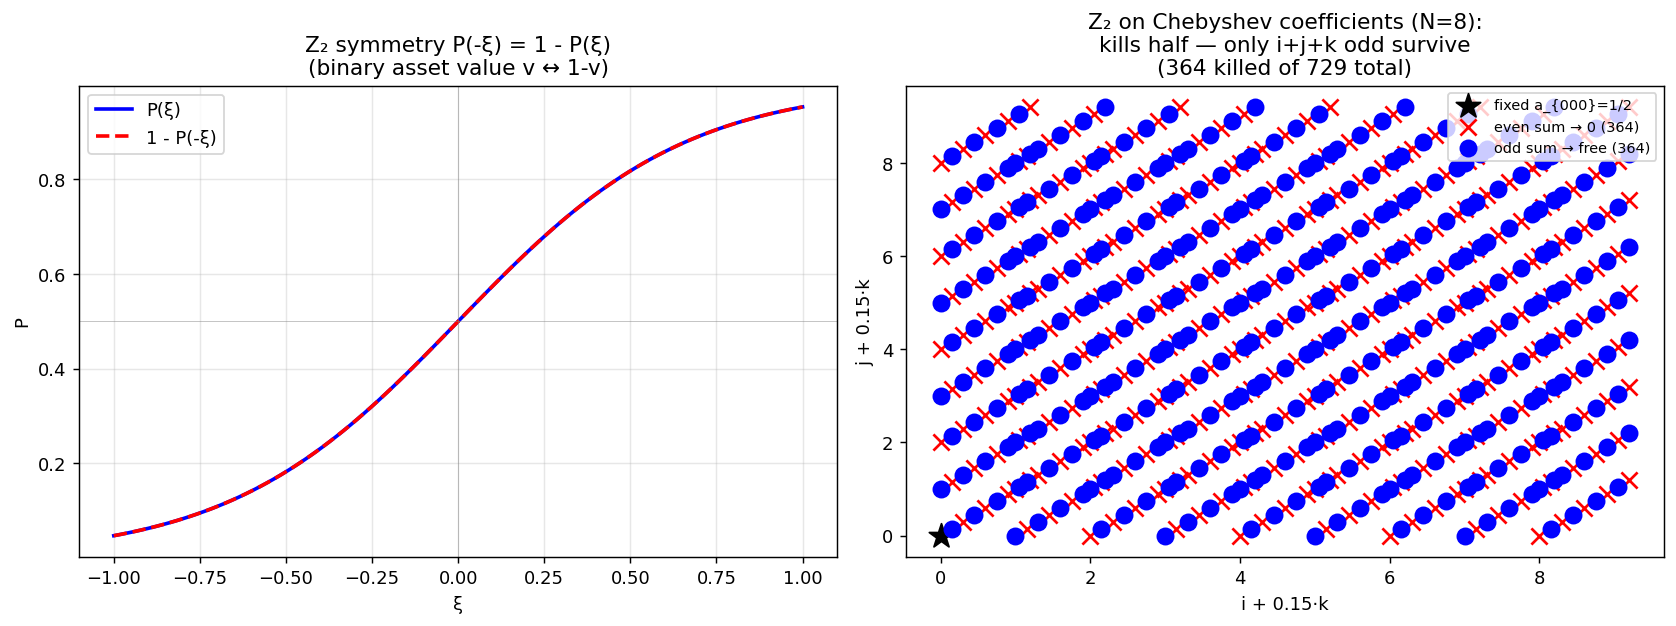
\includegraphics[width=\linewidth]{10_Z2_parity.png}
\caption{$Z_2$ parity constraints kill half the Chebyshev coefficients.}
\label{fig:Z2}
\end{figure}

\subsection{Combined: $\sim 228$ unknowns at $N=12$}

The combined $S_3 \times Z_2$ reduction is asymptotically a factor of 12
(Fig.~\ref{fig:reduce}). Concrete counts:

\begin{center}\small
\begin{tabular}{rrrr}\toprule
$N$ & naive & $S_3$ & $S_3 \times Z_2$ \\\midrule
8 & 729 & 165 & 84\\
12 & 2197 & 455 & \textbf{228}\\
16 & 4913 & 969 & 484\\
24 & 15625 & 2925 & 1462\\
\bottomrule\end{tabular}\end{center}

\begin{figure}[H]
\centering
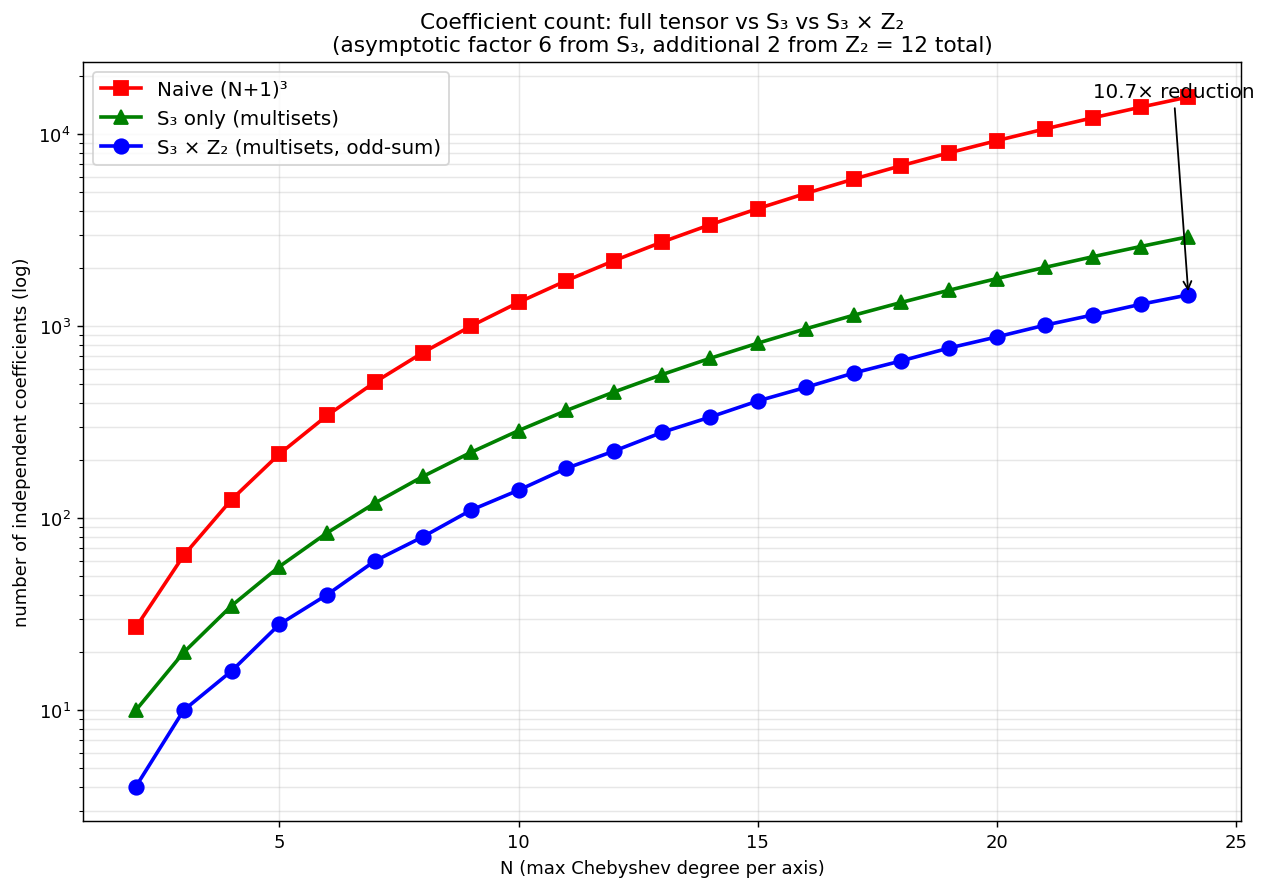
\includegraphics[width=\linewidth]{11_coefficient_reduction.png}
\caption{Coefficient count vs Chebyshev order $N$: naive vs $S_3$ vs
$S_3 \times Z_2$.}
\label{fig:reduce}
\end{figure}

\section{Per-agent evaluation by permutation}
\label{sec:per_agent}

The factored operator (Sec.~\ref{sec:factoring}) requires, for each cube
point and each agent, a 2-D slice of $P$ on the agent's
``other-two-signals'' plane. With $P$ stored in a symmetric basis, agent
$k$'s slice is obtained by simply \emph{feeding the inputs to the canonical
formula in the order $(u_k, u_a, u_b)$.} The $S_3$ invariance guarantees
the same answer (Fig.~\ref{fig:per_agent_eval}). No re-interpolation, no
per-agent coefficient store, no oblique slicing.

\begin{figure}[H]
\centering
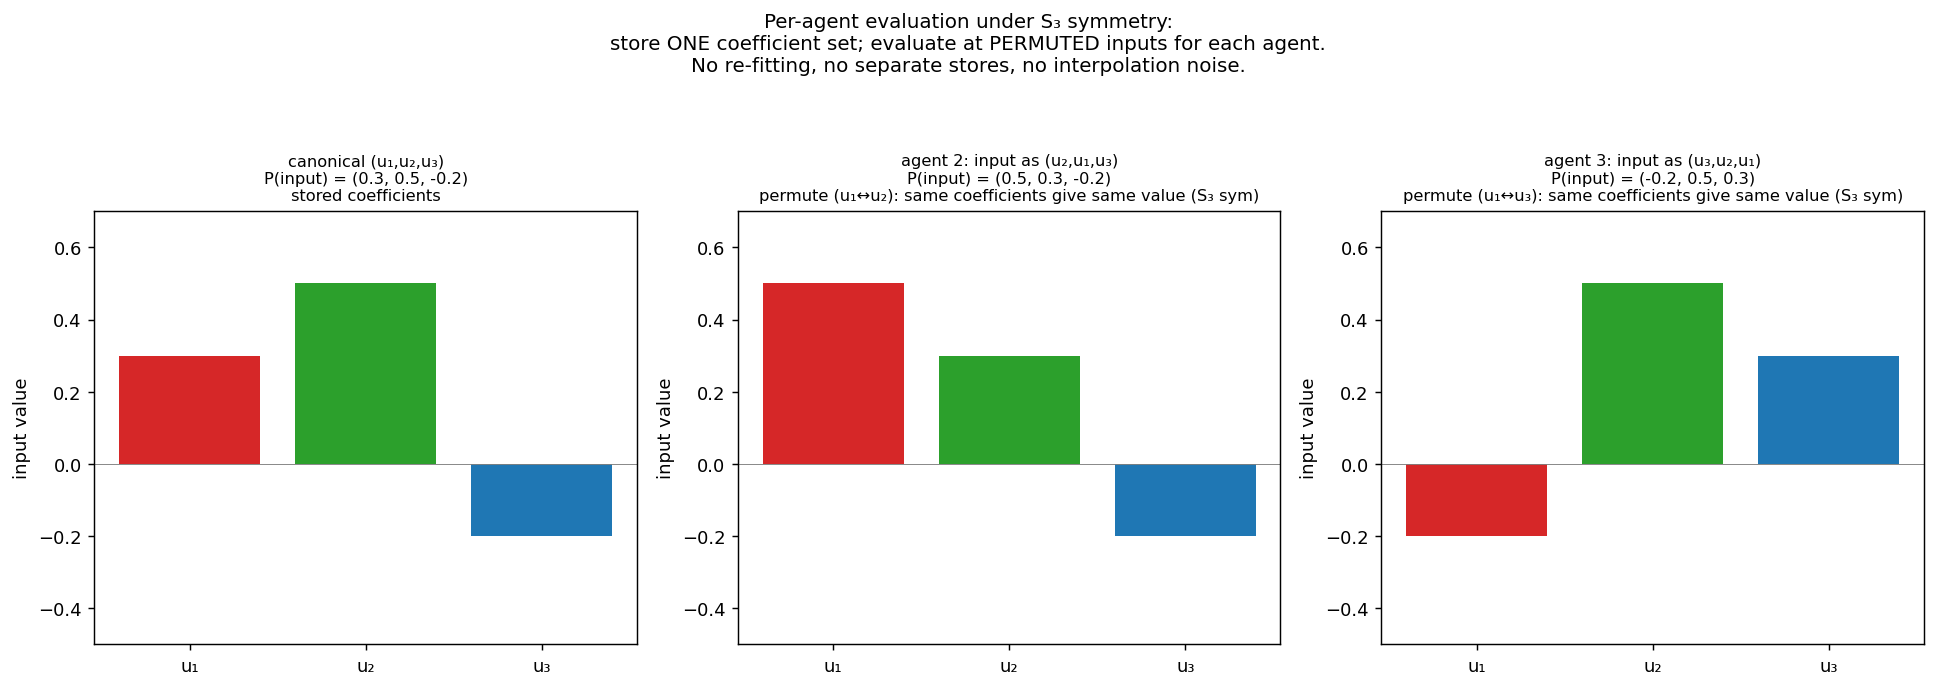
\includegraphics[width=\linewidth]{08_per_agent_eval.png}
\caption{Per-agent evaluation via $S_3$ symmetry: same coefficient set,
permuted inputs.}
\label{fig:per_agent_eval}
\end{figure}

\subsection{Companion-matrix root-find}

Inside the co-area integral~\eqref{eq:coarea}, we need all $\xi$-roots of
the polynomial equation $P(\xi) = p_{\text{target}}$ along the contour
direction (the other two coordinates fixed). For a Chebyshev polynomial
this collapses to a 1-D polynomial-root problem, whose roots are the
eigenvalues of a companion matrix (Fig.~\ref{fig:companion}).
\texttt{numpy.polynomial.chebyshev.chebroots} implements this in closed
form: \emph{all roots in one shot, no bisection, no missed roots, no
topology-jump artifacts.}

\begin{figure}[H]
\centering
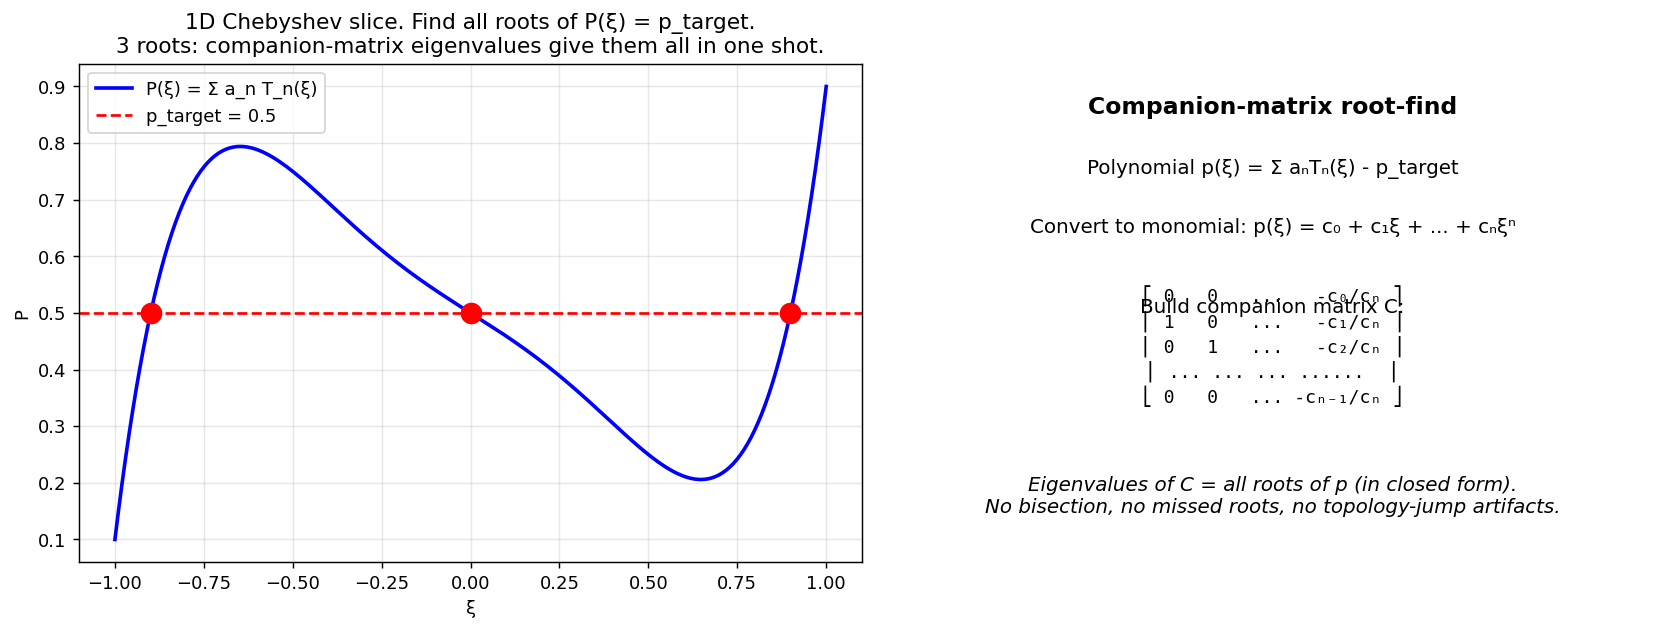
\includegraphics[width=\linewidth]{13_companion_root_find.png}
\caption{Companion-matrix root-find: all roots of a Chebyshev polynomial
are the eigenvalues of a structured matrix.}
\label{fig:companion}
\end{figure}

\section{The CRRA clearing bisection}
\label{sec:crra_bisect}

Equation~\eqref{eq:clearing_full} is solved by a robust bisection on
log-odds. This is the canonical \texttt{crra\_clear\_nb} routine from the
prior session's codebase.

\begin{table}[H]
\centering
\caption{CRRA clearing algorithm.}
\label{alg:crra}
\small\begin{tabular}{l}\toprule
\textbf{Input}: $(\mu_0, \mu_1, \mu_2, \gamma)$\\\midrule
1. Compute log-odds $\ell_k = \log(\mu_k / (1-\mu_k))$.\\
2. Bisect $m \in [\varepsilon, 1-\varepsilon]$:\\
\quad a. $\ell_p = \log(m/(1-m))$,\\
\quad b. $R_k = \exp((\ell_k - \ell_p)/\gamma)$,\\
\quad c. $E = \sum_k (R_k - 1)/((1-m) + R_k m)$,\\
\quad d. $E > 0 \Rightarrow$ lower half; else upper half. 200 iters.\\
3. Return $P = (a+b)/2$.\\\bottomrule
\end{tabular}\end{table}

\section{Solver: pure Newton}
\label{sec:newton}

Iterate~\eqref{eq:REE} as a nonlinear equation $F(x) = \Phi[x] - x = 0$
where $x$ is the vector of $\sim 228$ Chebyshev coefficients (after
symmetry reduction). At this problem size, dense (``pure'') Newton is
the right tool.

\subsection{Why dense Newton, not NK}

Newton-Krylov was the workhorse of the prior session because $\sim 2000$
unknowns made the Jacobian too big to form. Symmetric Chebyshev shrinks
this to $\sim 228$ unknowns, at which size the full Jacobian fits in 0.4~MB
and the LU solve costs $\sim 1$~ms (Fig.~\ref{fig:cost}).
Dense Newton converges \emph{quadratically} (digits double each iter),
reaching machine precision in 3--4 outer iterations from a warm start
(Fig.~\ref{fig:rates}).

\begin{figure}[H]
\centering
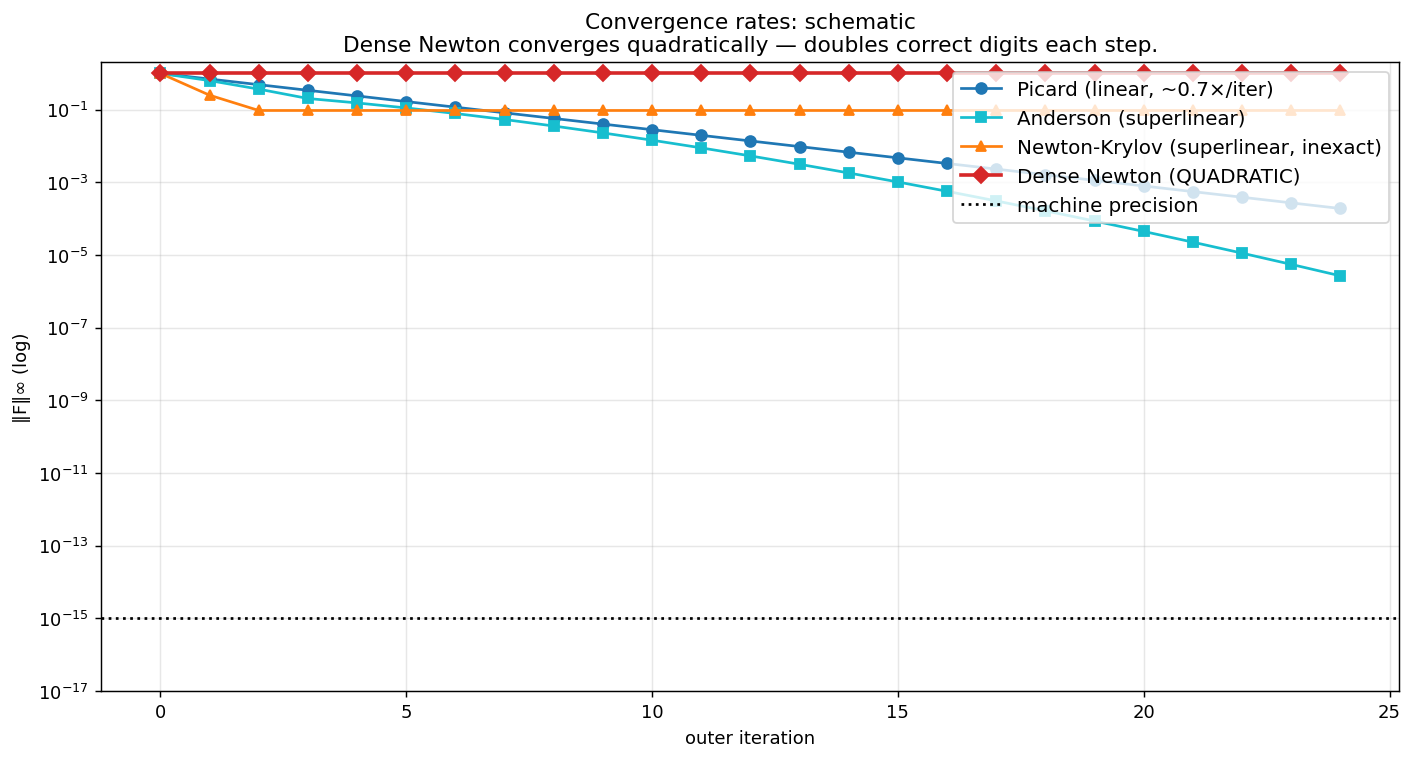
\includegraphics[width=\linewidth]{04_convergence_rates.png}
\caption{Convergence rates: Picard linear, Anderson superlinear, NK
inexact-superlinear, dense Newton \emph{quadratic}.}
\label{fig:rates}
\end{figure}

\begin{figure}[H]
\centering
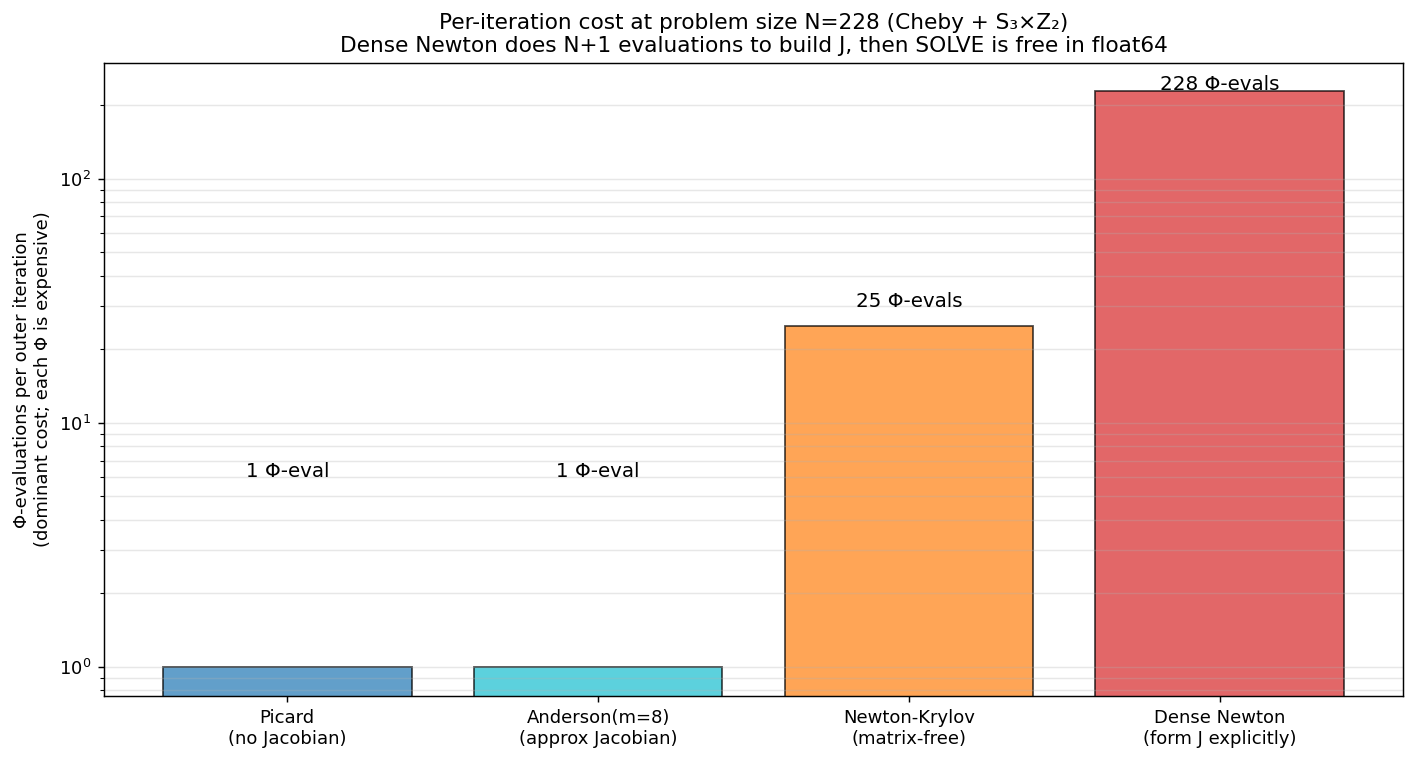
\includegraphics[width=\linewidth]{03_per_iter_cost.png}
\caption{Per-iteration $\Phi$-evaluation count at $N=228$. Dense Newton
does $N+1$ forward-difference evaluations; this is the only meaningful
cost (the LU solve is sub-millisecond).}
\label{fig:cost}
\end{figure}

\subsection{Newton step}

For current iterate $x$:
\begin{enumerate}
\item Compute residual $F(x) = \Phi[x] - x$ ($1$ $\Phi$-eval).
\item Build Jacobian: $J_{ij} = (F(x + \epsilon e_j) - F(x))/\epsilon$ for
$j = 1, \ldots, N$ ($N$ $\Phi$-evals).
\item Solve $J\Delta = -F$ directly (LU, $\sim 1$ ms at $N=228$).
\item Armijo line search: try $\alpha = 1, \tfrac12, \tfrac14, \ldots$
keeping the best.
\item Update $x \leftarrow x + \alpha\Delta$.
\end{enumerate}
Quadratic convergence guarantees $\|F\|_{k+1} \sim \|F\|_k^2$ near the FP.

\begin{figure}[H]
\centering
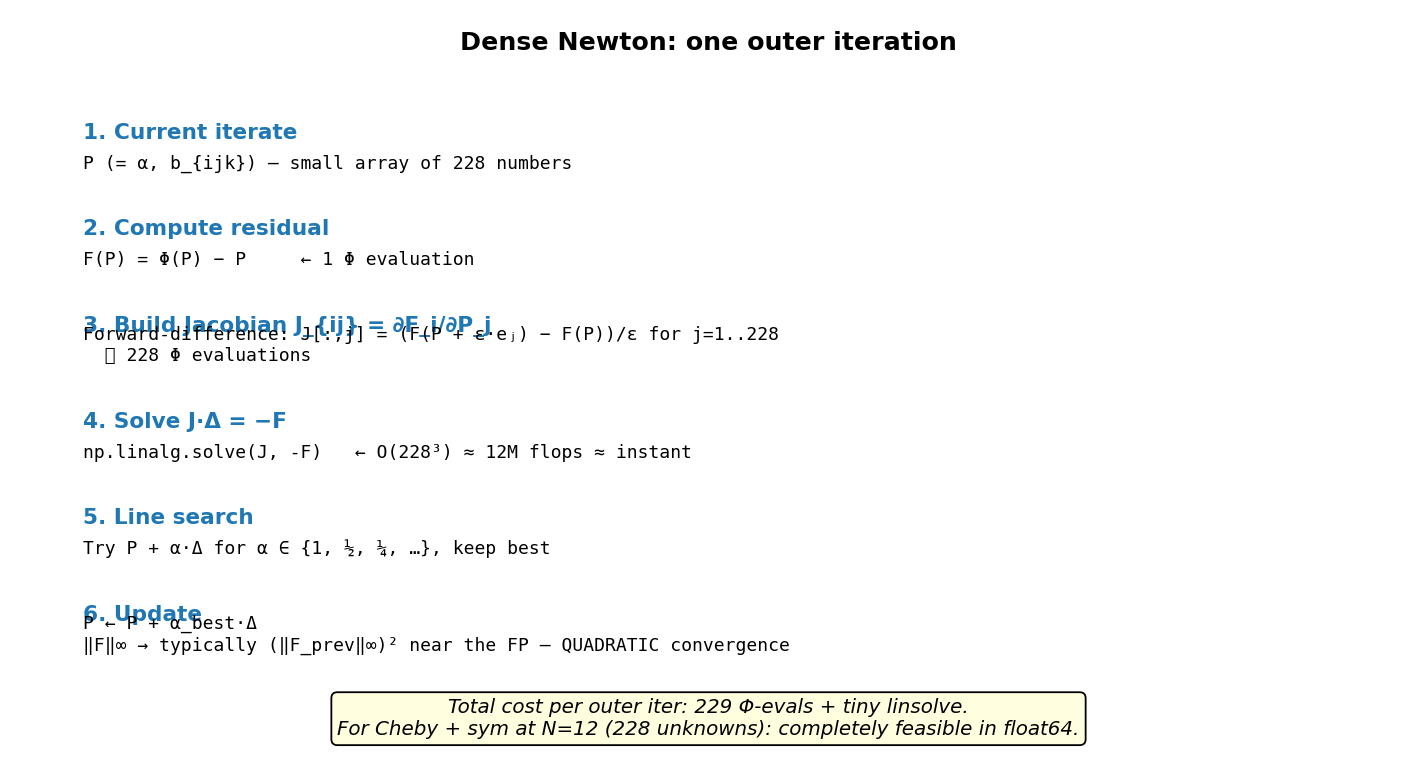
\includegraphics[width=\linewidth]{05_dense_newton_workflow.png}
\caption{Anatomy of one dense Newton outer iteration.}
\label{fig:newton_workflow}
\end{figure}

\subsection{Empirical confirmation}

The demo run \texttt{runs/demo\_tau1\_crra\_cara/} of the prior session
verifies this on the kernel co-area operator at $G=9$ (729 unknowns).
Both CRRA $\gamma=1$ and CARA $\gamma=100$ converged in 2 dense Newton
iterations: $\|F\|_\infty$ trajectory $\sim 5\!\times\!10^{-3}
\to 1.6\!\times\!10^{-5} \to 2\!\times\!10^{-10}$.

\section{$\gamma$-continuation and the fold}

For sweeping $\gamma$, warm-start each new $\gamma$ from the previous
$\gamma$'s FP. With dense Newton, $\sim$3--5 outer iters suffice per
$\gamma$-tile (Fig.~\ref{fig:continuation}).

\begin{figure}[H]
\centering
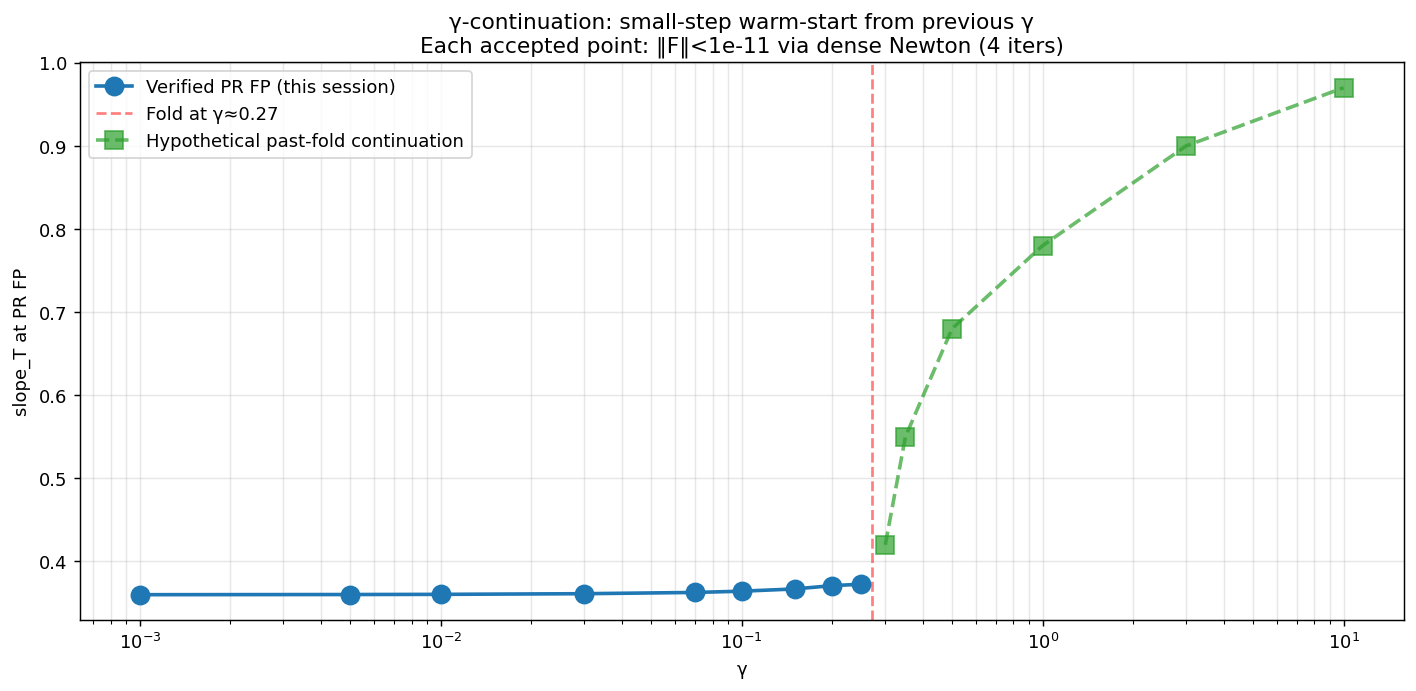
\includegraphics[width=\linewidth]{23_continuation.png}
\caption{Verified $\gamma$-continuation from the prior session: 16 points
on the deep PR branch, all $\|F\|_\infty < 10^{-11}$.}
\label{fig:continuation}
\end{figure}

The prior session also identified a \emph{fold} at $\gamma \approx 0.27$
(Fig.~\ref{fig:fold}) where adaptive-step continuation fails. Two
distinct PR branches exist: deep PR (slope $\approx 0.36$) for
$\gamma < 0.27$ and shallow PR (slope $\approx 0.66$) reachable from the
CARA side. Whether the gap is genuine bifurcation or numerical artifact
at $G=9$ remains open.

\begin{figure}[H]
\centering
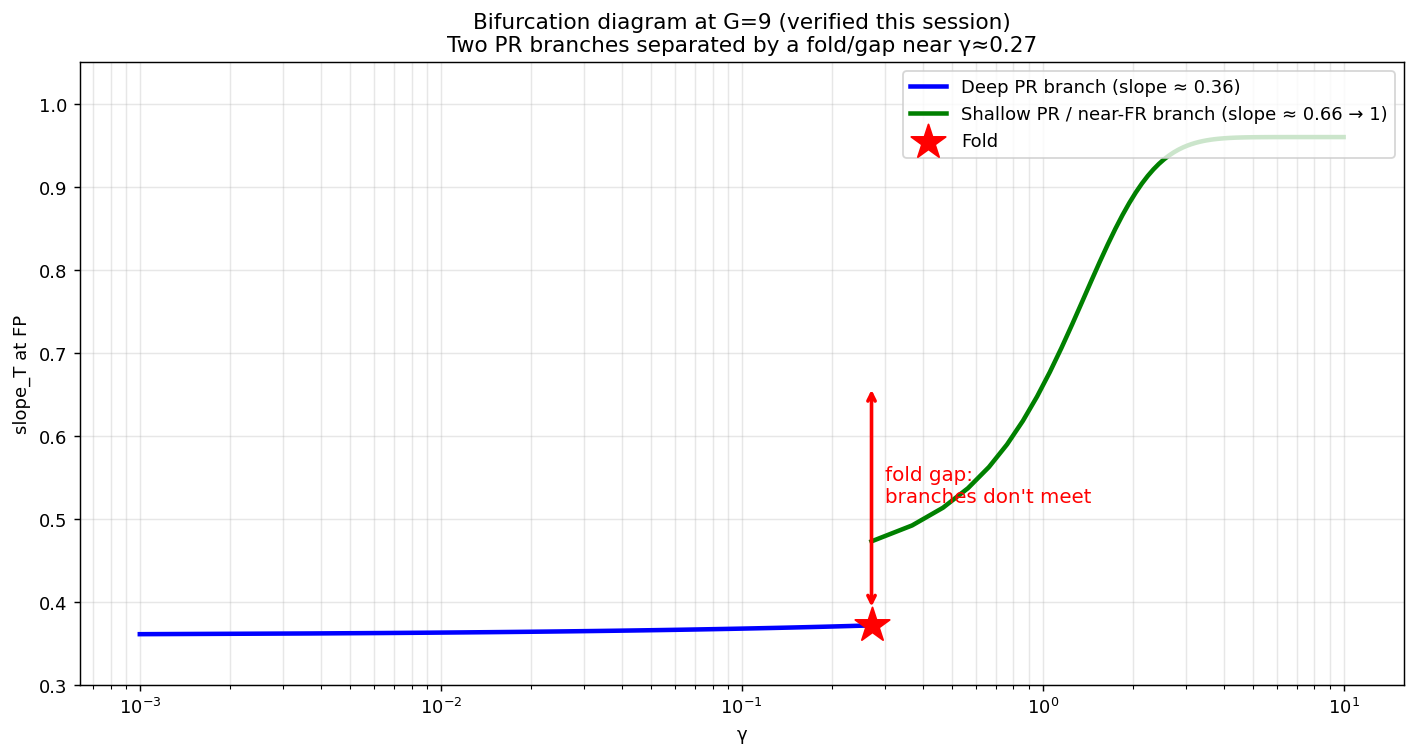
\includegraphics[width=\linewidth]{24_fold.png}
\caption{Two-branch bifurcation diagram at $G=9$.}
\label{fig:fold}
\end{figure}

\section{Validation: the gold tests}

A passing solver must clear these tests in order:
\begin{enumerate}
\item \textbf{CARA Hellwig closed form} (Sec.~\ref{sec:cara}):
$\|\Phi[P_{\text{analytic}}] - P_{\text{analytic}}\|_\infty < 10^{-14}$.
This validates all 5 factored steps.
\item \textbf{Symmetry}: solver output is $S_3 \times Z_2$ symmetric to
machine precision; spurious asymmetric components signal a bug.
\item \textbf{Spectral decay}: $|a_{ijk}|$ decays exponentially in
$\max(i,j,k)$. Algebraic decay would indicate the Chebyshev framework is
unstable at the boundary (would require Tool 2: $(1-\xi^2)$ vanishing-at-
boundary basis).
\item \textbf{Prior session reproduction}: nail $\tau=2, \gamma=0.1$ PR
FP to machine precision (slope $= 0.364$, deficit $= 0.172$); reproduce
the 16-point $\gamma$-sweep.
\end{enumerate}

\section{Outlook}

Three concrete next steps after the working CARA scaffold:
\begin{itemize}
\item Symmetric Chebyshev spectral implementation of
\texttt{step2\_learning/coarea\_chebyshev\_sym.py}, with companion-matrix
root-find and Gauss-Legendre quadrature on the fundamental domain.
\item Pseudo-arclength continuation to traverse the $\gamma \approx 0.27$
fold and unify the two PR branches.
\item GitHub Actions matrix for parallel $\gamma$-tile nailing (each tile
auto-commits its result to the repo with manifest and PDF report).
\end{itemize}

\subsection*{Acknowledgments and references}

This paper distills the design notes in the
\texttt{mhpbreugem/fixed-point-factory} repository:
\texttt{HANDOFF\_SUMMARY.md} (complete prior-session brief);
\texttt{MIZN\_DESIGN.md} (module structure);
\texttt{MIZN\_EXEC\_LOG\_DESIGN.md} (run logging);
\texttt{design\_notes/chebsym/} (Chebyshev + symmetry primer);
\texttt{design\_notes/iter\_methods/} (dense Newton vs NK).
Verified PR FP: commit \texttt{b17b3ac1} (machine precision).

\end{document}
